\documentclass[10pt,twocolumn,letterpaper]{article}

\usepackage{cvpr}
\usepackage{times}
\usepackage{epsfig}
\usepackage{graphicx}
\usepackage{amsmath}
\usepackage{amssymb}
\usepackage{enumitem}
\usepackage{float}

\graphicspath{{./images}}
% Include other packages here, before hyperref.

% If you comment hyperref and then uncomment it, you should delete
% egpaper.aux before re-running latex.  (Or just hit 'q' on the first latex
% run, let it finish, and you should be clear).
\usepackage[pagebackref=true,breaklinks=true,letterpaper=true,colorlinks,bookmarks=false]{hyperref}
\cvprfinalcopy % *** Uncomment this line for the final submission

\def\cvprPaperID{****} % *** Enter the CVPR Paper ID here
\def\httilde{\mbox{\tt\raisebox{-.5ex}{\symbol{126}}}}

% Pages are numbered in submission mode, and unnumbered in camera-ready
\ifcvprfinal\pagestyle{empty}\fi
\begin{document}

%%%%%%%%% TITLE
\title{Machine Learning Research Project}

\author{George Katsonis\\
American College of Thessaloniki\\
% Institution1 address\\
{\tt\small giorgos\_katsonis@hotmail.com}
}

\maketitle
%\thispagestyle{empty}

%%%%%%%%% ABSTRACT
\begin{abstract}
   In this paper we introduce the basics of machine learning research in the field of image classification. First, we describe the relevant metrics that are used to evaluate model performance. Next, we present a brief overview of a number of important data-sets used for various image classification tasks. Finally, we present our model utilizing inception convolution modules in order to achieve 86\% validation accuracy in CIFAR10, and going through the experimentation procedure, outlining possible future improvements.
\end{abstract}

%%%%%%%%% BODY TEXT
\section{Introduction}
\subsection{Metrics}
The most commonly used metrics for the calculation of the performance of a machine learning algorithm are the average accuracy, the F1-score, the top-k error, and the confusion matrix. \cite{iba_deep_2020}

\subsubsection{Average accuracy}
 The average accuracy is the number of correct predictions divided by the number of samples, it can be represented both as a fraction and as a percentile, though the latter is most common.
 
\subsubsection{F1-score}
The F1-score correlates the opposing metrics of precision and recall using the following formula:

\[
    {F1} = 2 * \frac{1}{\frac{1}{precision} + \frac{1}{recall}}
\]

\noindent Where:
\begin{itemize}[leftmargin=*]
    \item \textbf{Precision}: The number of true positive results divided by the predicted positive results.
    
    \[
    {Precision} = \frac{True Positives}{{True Positives} + {False Positives}}
    \]
    
    \item \textbf{Recall}: The number of true positive results divided by all the results that should have been predicted as positive.
    
    \[
    {Precision} = \frac{True Positives}{{True Positives} + {False Negatives}}
    \]
\end{itemize}

\subsubsection{Confusion Matrix}
 The confusion matrix is not only useful as a metric for performance but also as a visualization. It is a table where one dimension is all the actual labels, and the other is all the predictions of the model. For every sample, an overlap between the label on x and the label on y is a correct prediction. When constructing a confusion matrix, a diagonal is created that contains the overlaps, and thus the correct predictions. This allows us to easily see not only how many mistakes our algorithm made, but also allows us to identify clusters of incorrect predictions that might be caused by relations inside our data \cite{iba_deep_2020}.
 
\subsubsection{Top-k error}
The top-k error is a score that increases when the correct label is included in the top k predictions of the model based on probability. This means that for a top-1 error we will have an increase in score only if the top predicted class of the model is the correct one, while for a top-5 error it suffices for the correct label to be one of the top 5 predicted. Clearly, the larger the k, the easier it becomes to score high, and the more meaningless the score becomes.

\subsection{Data-sets}
In machine learning we see two types of research. The first is application-oriented research, where the paper will attempt to create a solution to a specific problem using machine learning. The second is generalized research, where the paper will push the state-of-the-art models in order to improve them, using standardized benchmarks to demonstrate the improvements. Application-oriented research often uses specialized data-sets relevant to the examined domain.

\subsubsection{TrashNet}
 TrashNet \cite{karthikeyan_review_2022} is a data-set used in waste classification. It contains 2527 images, taken from mobile devices, and categorized as:  glass, paper, cardboard, plastic, metal, and trash. As most domain-specific data-sets, TrashNet is extremely small; however, a number of techniques, that will be discussed later, are used to increase the sample number. In this paper we will be focusing on generalized research data-sets. These data-sets usually contain a large number of samples and features, they are extremely well documented, and often have many variants, curated versions of the original data-set that caters to a specific learning requirement. 

\subsubsection{CIFAR}
CIFAR \cite{iba_deep_2020} \cite{sankar_regularizing_2017} \cite{wang_residual_2017} is perhaps the most well-known families of data-sets for image classification machine learning research. The most popular variants are the original CIFAR 100 and its predecessor CIFAR 10. CIFAR 10 \cite{noauthor_cifar-10_nodate} consists of 60000 32x32 color images divided equally in 10 classes. CIFAR 100 \cite{noauthor_cifar-100_nodate} while having the same number of samples and the same resolution as its predecessor, greatly increases the number of classes to 100. The 100 classes are equally divided to 20 super classes providing more general categorization. For example, the classes beaver, dolphin, otter, seal, and whale are part of the superclass aquatic mammals. Caltech 256, much like CIFAR 100, is a direct increase on Caltech 101’s size and complexity. It contains 30,607 color images of different sizes, categorized unequally in 256 object classes and one additional clutter class, with each class containing at least 80 samples \cite{noauthor_caltech_nodate}. 

\subsubsection{MNIST}
MNIST is a very popular education and benchmarking data-set comprised of 70.000 images of handwritten digits. As a modified subset of NIST special databases 3 and 1, MNIST samples have been subjected to several normalization techniques in order to achieve a unified 29x29 grayscale resolution \cite{noauthor_papers_nodate}. The most interesting aspect of this data-set is the amount of variants that share its name. The largest variant of MNIST is Fashion MNIST \cite{noauthor_fashion_nodate}, a data-set of the same size and sample resolution as the original, meant to be a direct replacement of the original by its creator. The images in Fashion MNIST are of articles of clothing and the classes (remaining 9 as the digit classes of the original MNIST) are general clothing categories such as bag or trouser. MRDBI, or MNIST with Rotated Digits plus Background Images, dramatically increases the complexity of the original data-set in order to challenge the training models. Apart from the changes in the images indicated by the name, another factor of increased difficulty is the unusual split of the data to 12.000 training samples and 50.000 testing samples \cite{iba_deep_2020}.  Other less known variants of MNIST include Chinese MNIST \cite{noauthor_chinese_nodate}, which is comprised of 15.000 64x64 images of hand-drawn Chinese numbers, and sign language MNIST [16], a collection of 34627 24x24 grayscale samples representing hand signs categorized in 25 classes, one for each letter with no cases for 9=J and 25=Z since they require motion gesturing. 
The variants of MNIST are exceptionally different from the original; however, most generalized data-sets like CIFAR contain a very large number of variations created by slightly altering the images (i.e., flipping, mirroring, adding noise or distortion and even altering the colors). These techniques allow for exponentially increasing the number of samples in a data-set, or training models in specific ways \cite{he_deep_2015} \cite{zeiler_visualizing_2013}.

\subsubsection{ImageNet}
ImageNet \cite{krizhevsky_imagenet_2012} was the leading competition in image classification with machine learning. Despite the discontinuation of the competition, the benchmark data-sets used to facilitate it remain and are still widely used. Being perhaps the largest collection of labeled images, ImageNet contains over 15 million labeled high resolution pictures belonging to approximately 22,000 categories. Due to how vast the complete data-set is, there exist many subsets in order to make usage more accessible. One of those data-sets is the one used in the ImageNet Large-Scale Visual Recognition Challenge (ILSVRC). It contains approximately 1000 images in each category for a 1.2 million total training images, 50,000 validation images, and 150,000 testing images.

\subsubsection{Benchmark data-sets}
Due to the increasing rate of production for state-of-the-art models, there is a high demand for more streamlined and robust benchmarking solutions. Researchers \cite{lin_clear_2021} \cite{lomonaco_core50_2022} \cite{caldeira_image_2020} \cite{yellamraju_benchmarks_2018}create methodologies and data-sets that are meant to be used for the comparison of the performance for machine learning models for image classification. \cite{caldeira_image_2020}


\section{Proposed Model}
\subsection{Inception}
The model we propose utilizes inception modules for convolutions instead of the baseline. An inception module consists of 5 layers, excluding the input layer. Those are:
\begin{itemize}
    \item 1x1 convolution.
    \item 3x3 convolution.
    \item 5x5 convolution.
    \item 3x3 max pooling.
    \item Concatenation Layer.
\end{itemize}

The operations in the convolution and max pooling layer run independently and the resulting maps are concatenated to produce a single output. As shown in figure \ref{fig:inc}. \cite{szegedy_going_2014}
\begin{figure}[h]
\centering
\label{fig:inc}
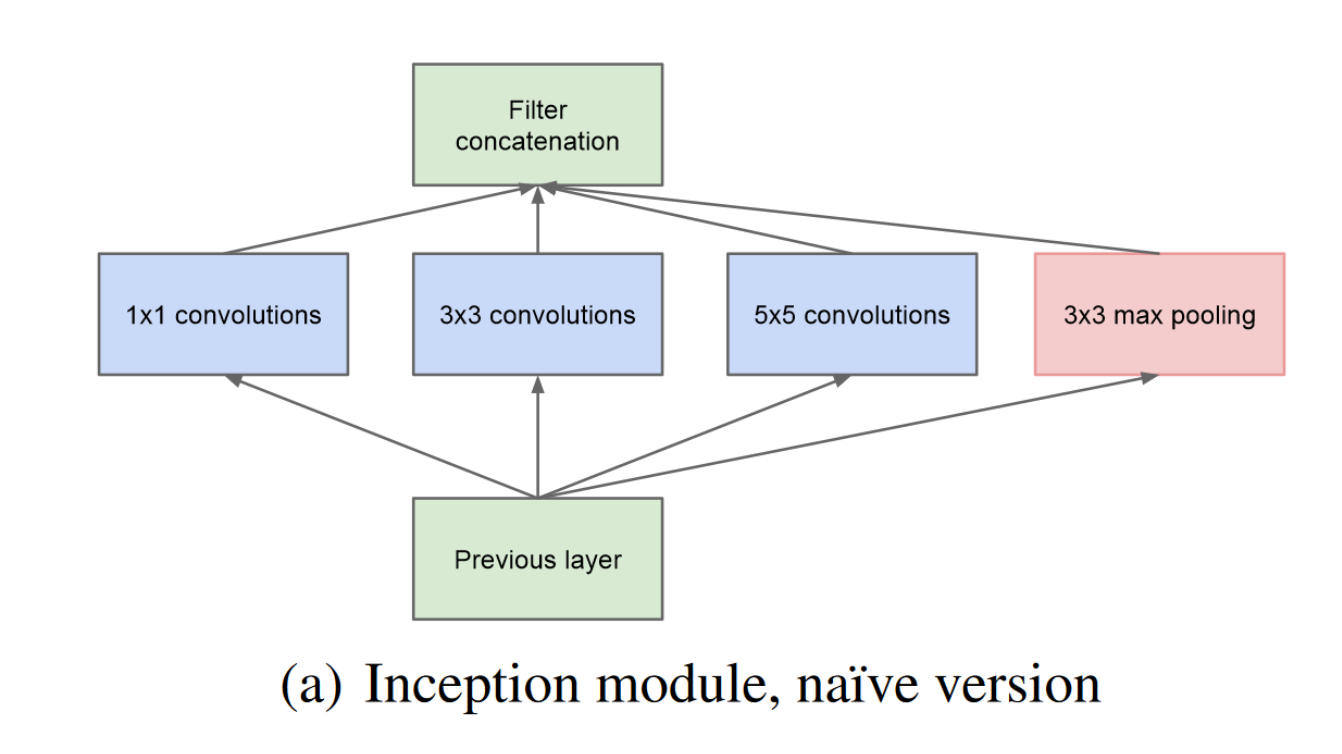
\includegraphics[scale = 0.23]{naive_inc.png}
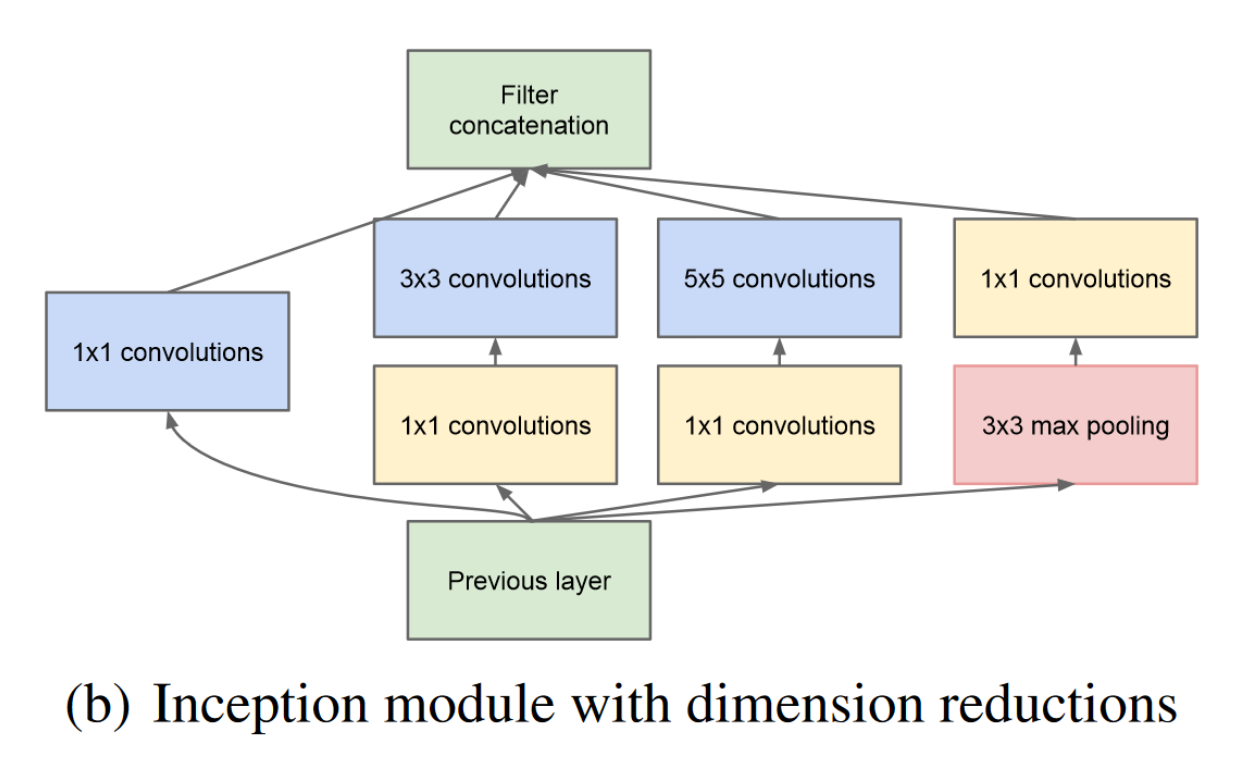
\includegraphics[scale = 0.25]{inception_module.png}
\caption{Inception modules}
\end{figure}

\subsection{Architecture - Data Flow}
\begin{table}[h!]
\centering
\begin{center}
\begin{tabular}{|l|c|}
\hline
Layer & Feature Number \\
\hline\hline
2D Convolution & 864 \\
ReLU & - \\
Batch normalization & 128 \\
2D Convolution & 9,216 \\
ReLU & - \\
Batch normalization & 128 \\
Inception 1 & 19,968\\
Dropout & -\\
Inception 2 & 24,064\\
Inception 3 & 82,944\\
Inception 4 & 329,728\\
Inception 5 & 1,314,816\\
Global average pooling 2D & -\\
Dropout & -\\
Dense & 7690\\
Softmax & -\\
Total Features & 1,789,546\\
\hline
\end{tabular}
\end{center}
\caption{Model architecture}
\end{table}

\begin{table}[H]
\centering
\begin{center}
\begin{tabular}{|l|c|}
\hline
Configuration & Value \\
\hline\hline
Padding Size & 1 \\
Window Size & 3 \\
Stride & 1 \\
Bias & None \\
Dropout Rate & 0.4 \\
L2 Regularization & True \\
Weight Decay & 1e-4\\
\hline
\end{tabular}
\end{center}
\caption{Module Configuration Parameters}
\end{table}


\subsection{Hyperparameters}
\begin{table}[h!]
\centering
\begin{center}
\begin{tabular}{|l|c|}
\hline
Hyperparameter & Value \\
\hline\hline
Epochs & 50 \\
Batch Size & 128 \\
Starting learning rate & 0.05 \\
Momentum & 0.9 \\
Cost Function & Categorical Cross-entropy\\
Optimizer & Stochastic Gradient Descent\\
Kernel initializer & Glorot uniform\\
\hline
\end{tabular}
\end{center}
\caption{Model Hyperparameters}
\end{table}

\begin{table}[h!]
\centering
\begin{center}
\begin{tabular}{|l|c|}
\hline
Epochs & Learning Rate \\
\hline\hline
20 & 0.01 \\
40 & 0.005 \\
\hline
\end{tabular}
\end{center}
\caption{Learning Rate Schedule}
\end{table}

\subsection{Data processing}
The data has been standardized and some image augmentation has been implemented by randomly flipping the images. Random cropping was also attempted but never managed to reduce over-fitting, instead leading to overall worse performance for the model.

\subsection{Model Performance}

\begin{table}[h!]
\centering
\begin{center}
\begin{tabular}{|l|c|c|}
\hline
Model & Average Accuracy & F1-Score \\
\hline\hline
Baseline & 70\% & 0.7\\
Ours & 86\% & 0.861 \\
\hline
\end{tabular}
\end{center}
\caption{Model Comparison}
\end{table}

\begin{figure}[H]
\centering
\label{fig:acc}
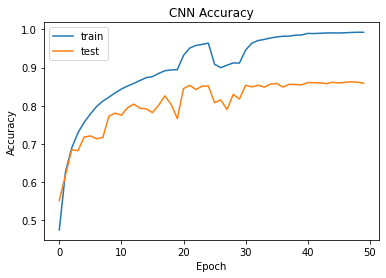
\includegraphics[scale = 0.6]{images/best_accuracy.png}
\caption{CNN Accuracy}
\end{figure}

\begin{figure}[H]
\centering
\label{fig:err}
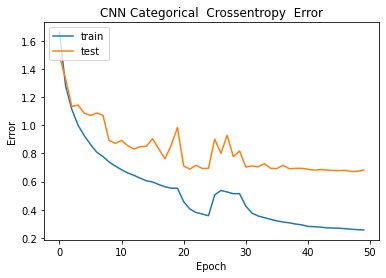
\includegraphics[scale = 0.6]{images/best_error.png}
\caption{CNN Error}
\end{figure}

\begin{figure}[H]
\centering
\label{fig:conf}
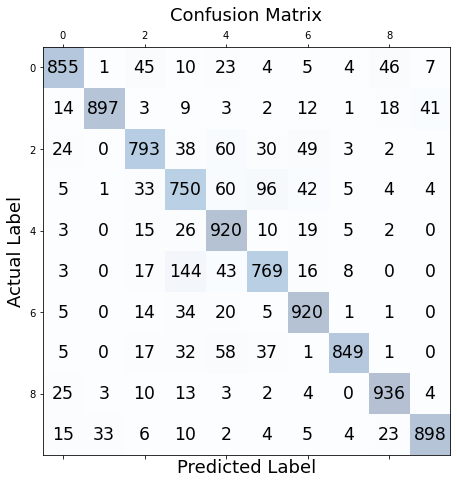
\includegraphics[scale = 0.45]{images/best_acc_conf_matrix.png}
\caption{Confusion Matrix }
\end{figure}

\section{Experiments}
For the detailed account of the experimentation process please view the \href{https://github.com/XarsEvandor/Machine-Learning-CIFAR10/blob/main/Captain's\%20Log.md}{timeline}. In this section we will outline some interesting observations, as well as an alternative model architecture.

\subsection{Observations}
\begin{itemize}
    \item Standardization did nothing to improve over-fitting over regular normalization.
    \item Removing, moving, or adding more dropout layers drastically reduced performance no matter the other parameters.
    \item Random cropping image augmentation led to worse performance when used both in terms of training accuracy as well as over-fitting.
    \item Google collab will revoke your right to use a GPU if you forget terminating the run-time, leading to you not having graphs for the alternative model.
    \item Trying to avoid local minima by temporarily increasing the learning rate using the scheduler does work, by reducing the accuracy sharply before it returns to the plateau.
    \item 86\% accuracy seems to be a hard limit for inception no matter the surrounding parameters.
\end{itemize}

\subsection{Alternative model}
\begin{table}[h!]
\centering
\begin{center}
\begin{tabular}{|l|c|}
\hline
Layer & Feature Number \\
\hline\hline
2D Convolution & 864 \\
ReLU & - \\
Batch normalization & 128 \\
2D Convolution & 9,216 \\
ReLU & - \\
Batch normalization & 128 \\
Inception 1 & 19,968\\
Dropout & -\\
Inception 2 & 24,064\\
Inception 3 & 82,944\\
Inception 4 & 95,232\\
Inception 5 & 329,728\\
Basic Convolutional & 442,880\\
Global average pooling 2D & -\\
Dropout & -\\
Dense & 1290\\
Softmax & -\\
Total Features & 1,006,442\\
\hline
\end{tabular}
\end{center}
\caption{Alternative Model architecture}
\end{table}

With this model we achieve 85.6\% accuracy while reducing the number of features by 700,000 making the model significantly faster.


\section{Conclusions}
In this paper we presented an overview of the core metrics and datasets for image classification problems. We have presented two models that significantly improve on the baseline model's accuracy by using inception modules. Finally, we have recorded the observations made during our experiments. Points for future research would be the implementation of a Res-Net module, the experimentation with different cost and activation functions, different optimisers, as well as the implementation of adaptive learning rates that increase when the model plateaus. 

%-------------------------------------------------------------------------

%-------------------------------------------------------------------------
\section{References}
{\small
\bibliographystyle{ieee}
\bibliography{proj}
}




\end{document}
